%&latex
\documentclass[a4paper]{article}

\usepackage{graphicx}
\usepackage[T1]{fontenc}
\usepackage[spanish]{babel}

\begin{document}

%+Title
\title{\textbf{Un algoritmo para reconocimiento de actividades humanas de dos fases en el ambito de la Industria 4.0 y procesos humanos dirigidos}
}

\author{Borja Bordel\(^{1}\), Ramón Alcarria\(^{1}\), Diego Sánchez-de-Rivera\(^{1}\)}
\date{\(^{1}\)Universidad Politécnica de Madrid, \begin{center}Madrid, España\end{center}}
\maketitle
%-Title

\begin{}
    \textbf{Resumen: }Futuros sistemas industiales, una revolución conocida como Industria 4.0, son visualizados para integrar a la gente en el mundo cibernetico como prsosumidores (proveedores de servicios y consumidores). En este contexto, los procesos impulsados por humanos aparecen como una realidad esencial y aparecen instrumentos para crear bucles de información de opiniones entre el subsistema social (personas) y el subsistema cibernético (componentes tecnológicos) son requeridos. Aunque muchos instrumentos distintos han sido propuestos, hoy en día las técnicas del patrón de reconocimiento son las más prometedoras. Sin embargo, estas soluciones presentan algunos  problemas pendientes. Por ejemplo, estas técnicas dependen de el hardware seleccionado para adquirir información de los usuarios; o presentan un límite en la precisión del proceso de reconocimiento. Para abordar esta situación, en este artículo se propone un algorítmo de dos fases para integrar a las personas en el sistema de la Industria 4.0 y los procesos impulsados por humanos. El algoritmo describe acciones complejas como composiciones de movimientos simples. Acciones complejas reconocidas usando los Modelos Ocultos de Markov, y los movimientos simples son reconocidos usando el Ajuste de Tiempo Dinámico. De esa manera, solo los movimientos son dependientes en el hardware de los dispositivos empleado para recolectar información, y la precisión del reconocimiento de acciones complejas mejora considerablemente. Una validación experimental real es también llevada a cabo para evaluar y comparar el rendimiento de la solución propuesta.
\begin{}\textbf{Palabras clave:} Industria 4.0; Patrón de reconocimiento; Ajuste de Tiempo Dinámico; Inteligencia Artificial; Modelos Ocultos de Markov.\end

    
    \end{abstract}
%-Abstract

%+Contents

%-Contents

\section{Introducción}
Industria 4.0 [1] hace referencia al uso de Sistemas Ciberfísicos (unión de procesos físicos y cibernéticos) [2] como el componente tecnológico principal en soluciones digitales futuras, principalmente (pero no únicamente) en escenarios industriales. Normalmente, la digitalización ha causado, al final, que los trabajadores en las líneas de ensamble fueran sustituidos por robots durante la tercera revolución industrial.
Sin embargo, algunas aplicaciones industriales no pueden basarse en soluciones tecnológicas, siendo el trabajo humano aún esencial [3]. Los productos hechos a mano son un ejemplo de las aplicaciones donde la presencia del trabajo humano es esencial. Estos sectores industriales, en cualquier caso, debe ser también integrado en la cuarta revolución industrial. De la unión de los Sistemas Ciberfísicos (CPS) y los humanos actuando como proveedores de servicio (trabajos activos), surgimiento del CPS humanizado [4]. En estos nuevos sistemas, los procesos antropogénicos son permitidos [5]; i.e. los procesos que son conocidos, ejecutados y manejados por personas (a pesar de que deben ser vigilados por mecanismos digitales).
Para crear una integración real entre personas y tecnología, y mover la ejecución del proceso del subsistema social (humanos) al mundo cibernético (componentes de hardware y software), las técnicas de la extracción de la información son necesarias. Muchas soluciones diferentes y acercamientos han sido reportados durante los últimos años, pero las técnicas de reconocimiento de patrones son las más prometedoras.
El uso de Inteligencia Artificial, modelos estadísticos y otros instrumentos similares han permitido un real e increíble desarrollo de soluciones de reconocimiento de patrones, pero algunos desafíos todavía siguen pendientes.
Primero, las técnicas de reconocimiento de patrones dependen del hardware subyacente para captar información. La estructura y los cambios en el proceso de aprendizaje si (por ejemplo) en vez de acelerómetros que  consideramos sensores infrarrojos. Esto es muy problemático debido a que las tecnologías de hardware evolucionan mucho más rápido que las soluciones de software.
Y, segundo, hay un límite en la precisión en el proceso de reconocimiento. En realidad, como las acciones humanas se vuelven más complicadas, más variables y más modelos complejos son requeridos para reconocerlos. Esta aproximación genera grandes problemas de optimización cuyo error residual es más alto según aumenta el número de variables; lo que lo que provoca una disminución en la tasa de éxito del reconocimiento [6]. En conclusión, las matemáticas (no el software, por lo que, no depende de la implementación) fuerza una cierta precisión para el proceso del reconocimiento de patrones haciendo que las acciones sean estudiadas. Para prevenir esta situación, se debe considerar un número más bajo de variables, pero esto también reduce la complejidad de las acciones que deben ser analizadas; una solución que no es aceptable en escenarios industriales donde las actividades de producción complejas son desarrolladas.
Por lo tanto, el objetivo de este artículo es describir un nuevo algoritmo de reconocimiento de patrones abordando estos dos problemas básicos. El mecanismo propuesto define las acciones como una composición de movimientos simples. Los movimientos simples son reconocidos usando las técnicas de la Deformación Dinámica del Tiempo (DTW) [7]. Este proceso es dependiente de un hardware concreto para captar la información; pero la DTW es muy flexible y actualizar el repositorio de patrones es suficiente para reconfigurar todo el algoritmo. Luego las acciones complejas son reconocidas como combinaciones de movimientos simples a través de los Modelos Ocultos de Markov (HMM) [8]. Estos modelos son totalmente independientes de las tecnologías de hardware, ya que sólo se consideran como acciones simples. Este acercamiento de dos fases también reduce la complejidad de los modelos, incrementando la precisión y la tasa de éxito en el proceso de reconocimiento.
El resto del artículo está organizado de esta manera: La sección 2 describe el estado del arte en el reconocimiento de patrones para las actividades humanas; la sección 3 describe la solución propuesta, incluyendo las dos fases definidas; la sección 4 presenta un validación experimental usando un escenario real y usuarios finales; y la sección 5 cierra el artículo. 

\section{El estado del arte en el patrón de reconocimiento}
Muchas técnicas de patrón de reconocimiento distintas para actividades humanas han sido informadas. Sin embargo, la mayoría de las propuestas comunes pueden ser clasificadas en cinco categorías basicas [9]:(i)Modelos Ocultos de Markov; (ii) Campo Aleatorio Condicional con Cadenas de Salto; (iii) Patrones Emergentes; (iv) Campo Aleatorio Condicional; y (v) Clasificadores Bayesianos.
\setlegtth{\parindent}{<}\begin{}De hecho, la mayoría de autores proponen el suo de Modelos Ocultos de Marcov (MOM) para modelar actividades humanas. MOM permite modelar acciones como cadenas de Markov [10][11]. Basicamente, MOM genera estados ocutos desde datos observables. En particular, el objetivo final de esta técnica es construir la secuenciade estados ocultos que encaja con cierta secuencia de datos. Para finalmente definir el modelo completo, MOM debe deducir desde los datos los parametros del modelo de na manera confiable. La Figura 1 muestra una representación esquematizada
sobre como MOM funciona. Cuando las actividades humanas son reconocidas, las acciones que componen las actividades son los estados ocultos, y las respuestas de un sensor son datos bajo estudio. MOM, además, permite el uso de tecnicas de aprendizaje considerando el conocimiento anterior sobre el modelo. Este aprendizaje es algunas veces esencial para ``inducir´´ todas las secuencias de datos posibles requeridas para calcular el MOM. Finalmente, es muy importante notar que el MOM aislado simple puede ser combinado para crear modelos más amplios y más complejos. 

\center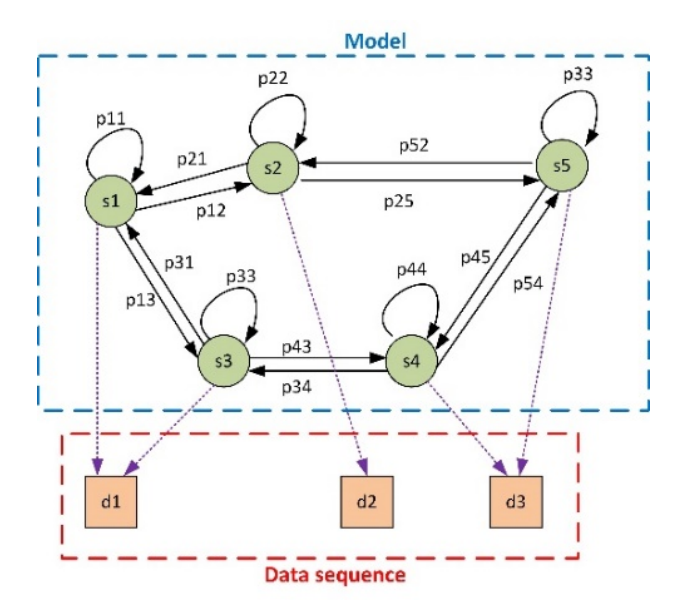
\includegraphics{Fig_1.png} 
\center\begin{}\textbf{Fig. 1.} Representación gráfica de un MOM
\setlegtth{\parindent}{<}\begin{}MOM, no obstante, son inútiles para modelar ciertas actividades concurrentes, así que otros autores han informado una nueva técnica llamada, Campo Aleatorio Condicional (CAC). CAC es uutilizado para modelar aquellas actividades que presentan acciones concurrentes o, en general, multiples acciones que interactuan [12][13]. Además, MOM requiere un gran esfuerzo en aprendizaje para descubrir todos los estados ocultos posibles. Para resolver estos problemas, el Campo Aleatorio Condicional (CAC) emplea probabilidades condicionales en vez de distribuciones de probabilidad unidas. De esa manera, las actividades cuyas acciones son desarrolladas en cualquier orden pueden ser facilmente modeladas. Contrariamente a las cadenas en MOM, CAC emplea gráficos acíclicos, y posibilita la integración de estados ocultos condicionales (estados que dependen de pasadas y/o futuras observaciones).
\setlegtth{\parindent}{<}\begin{}CAC, por otro lado, sigue siendo inútil para modelar ciertos comportamientos, así que algunas propuestas generalizan este concepto y proponen el Campo Aleatorio Condicional con Cadenas de Salto
(CACCS). CACCS es una técnica de patrón de reconocimiento, más general que CAC, que posibilita modelar actividades que no son de naturaleza de secuencias de acciones [14]. Esta técnica intenta capturar dependencias de largo rango (cadena de salto); y y podría ser entendido como el producto de diferentes cadenas lineales. Sin embargo, calcular este producto es bastante pesado y complicado, asi que esta técnica es normalmente demasiado computacionalmente cara para ser implementada en pequeños sistemas integrados. 
%+Bibliography
\begin{thebibliography}{99}
\bibitem{Label1} Bordel, B., Alcarria, R., Sánchez-de-Rivera, D., & Robles, T. (2017, Noviembre). 
Protegiendo los sistemas de la Industria 4.0 contra los efectos maliciosos de los ataques cyber-fisicos. En la Conferencia Internacional de Coputación ubicua y Inteligencia Ambiental (pp. 161-
171). Springer, Cham.
\bibitem{Label2} ...
\bibitem{Label3} ...
\bibitem{Label4} ...
\bibitem{Label5} ...
\bibitem{Label6} ...
\bibitem{Label7} ...
\bibitem{Label8} ...
\bibitem{Label9} ...
\bibitem{Label10} ...
\bibitem{Label11} ...
\bibitem{Label12} ...
\bibitem{Label13} ...
\bibitem{Label14} ...
\bibitem{Label15} ...
\bibitem{Label16} ...
\bibitem{Label17} ...
\bibitem{Label18} ...
\bibitem{Label19} ...
\end{thebibliography}
%-Bibliography

\end{document}


